\subsection{Arquitectura del Servidor}
El servidor está diseñado para manejar múltiples conexiones
simultáneas de clientes y procesar los datos recibos de los sensores
de manera eficiente. La arquitectura del servidor se basa en un modelo
cliente-servidor, donde el servidor actúa como el punto central de
comunicación y procesamiento de datos.


\begin{figure}[htb]
    \centering
    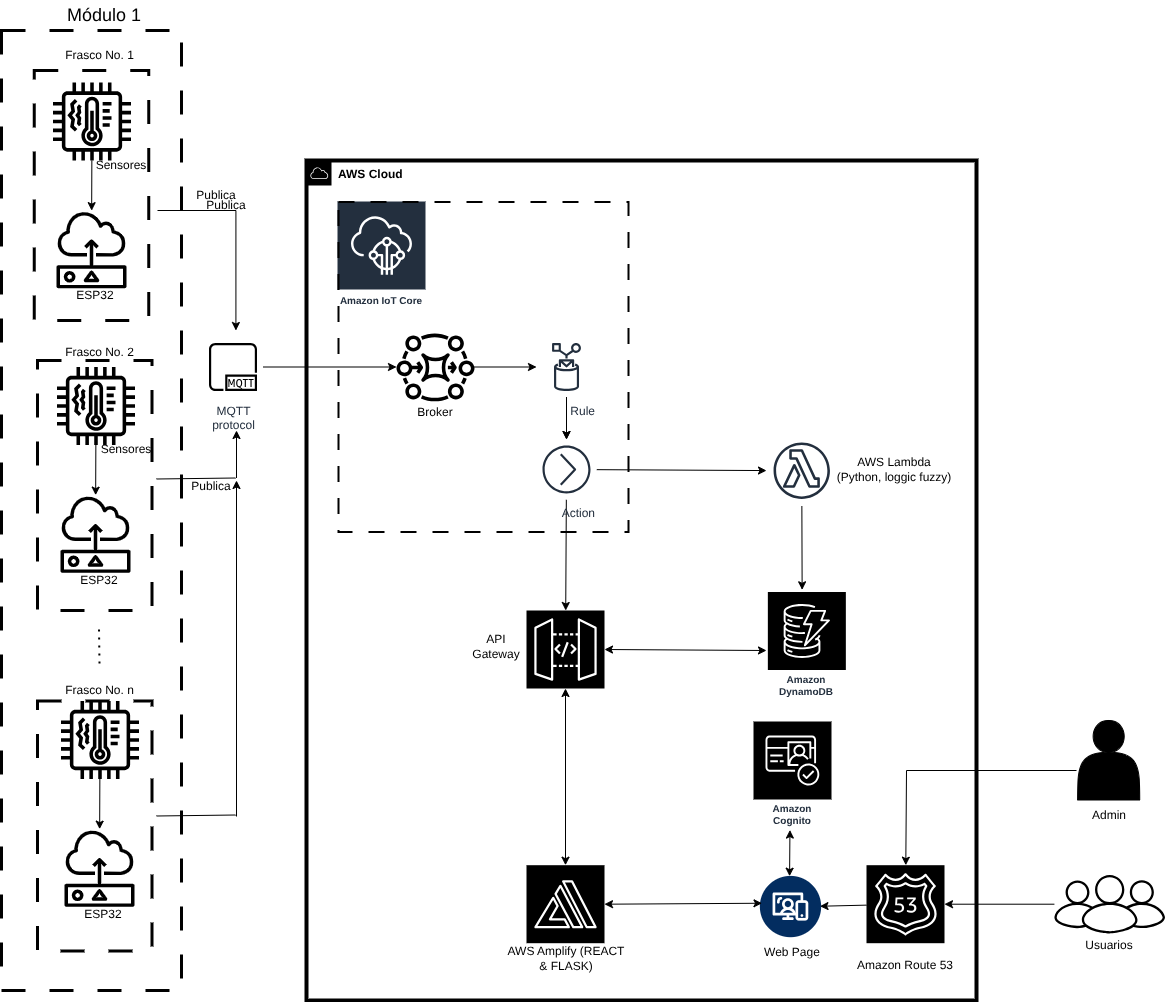
\includegraphics[width=1\textwidth]{./UML/Modulo4/arquitectura.drawio.png}
    \caption{Arquitectura del Servidor}
    \label{fig:Log1}
    \end{figure} 